\documentclass{article}
\usepackage{arxiv}

\usepackage[utf8]{inputenc} % allow utf-8 input
\usepackage[T1]{fontenc}    % use 8-bit T1 fonts
\usepackage{hyperref}       % hyperlinks
\usepackage{url}            % simple URL typesetting
\usepackage{booktabs}       % professional-quality tables
\usepackage{amsfonts}       % blackboard math symbols
\usepackage{nicefrac}       % compact symbols for 1/2, etc.
\usepackage{microtype}      % microtypography
\usepackage{lipsum}
\usepackage{graphicx}
\usepackage{caption}
\usepackage{subcaption}
\usepackage{float}
\usepackage[table,xcdraw]{xcolor}

\usepackage[linesnumbered,ruled]{algorithm2e}


\usepackage{amsmath}
\usepackage{amsthm}
\newtheorem{definition}{Definition}[section]
\newtheorem{theorem}{Theorem}[section]
\newtheorem{lemma}[theorem]{Lemma}
\newtheorem{hypothesis}{Hypothesis}
\theoremstyle{remark}

\title{Design and analysis of algorithms for Graph Packing Coloring}

\author{
  % Roy, Akash\thanks{Personal website: https://www.theroyakash.com} \\
  % Department of Computer Science \\
  % IIT Madras \\
  % \texttt{royakashappleid@icloud.com} \\
  Roy, Akash \\Dept. of Computer Science\\Indian Institute Of Technology, Madras\\\texttt{theroyakash@outlook.com} \and \textbf{Dr. B.V. Raghavendra Rao}\\Dept. of Computer Science\\Indian Institute Of Technology, Madras\\\texttt{bvrr@cse.iitm.ac.in}
}


\begin{document}
\maketitle

\begin{abstract}
In this report I discuss mathematical properties of a greedy heuristic I developed for the graph packing coloring problem. I discuss the motivation, design and analysis of an approximate coloring scheme for the packing coloring and explore its properties, compare approximation quality and discuss novelty in implementation.
\end{abstract}


\keywords{Algorithms \and Graph \and Graph Coloring \and Packing Coloring}


\section{Introduction}
 Let $G= (V,E)$ be an undirected graph. A vertex $k$ coloring of $G$ is a map $f: V \to \{1,\ldots, k\}$. A coloring $f$ is said to be proper, if for every edge $(u,v)\in E$, $f(u) \neq f(v)$. The chromatic number of a graph is the minimum value of $k$ such that $G$ has a proper $k$ colouring. 

Graph coloring is a widely studied concept in the area of graph theory with vast applications in computer science. For example,  proper colouring of planar graphs can be used to colour maps.  The graph colouring problem, i.e., obtaining a colouring of a graph with minimum number of colours has been widely studied by the algorithms research community for several decades.  While  the problem of determining if a given graph is three colorable or not is $\mathrm{NP}$-complete. There are several approximation algorithms for the problem.  

Given the centrality of graph colouring to graph theory and computer science, there have been several variants of colouring problems on graphs with some additional conditions imposed.  List coloring, path coloring, repetition free colouring are some of the prominent examples.  This thesis is concerned with a variant of distance based colouring known as packing coloring, more generally $S$-packing colouring. We  begin with a definition of the  graph packing-coloring problem.

\begin{definition}[\textit{$S$-Packing Coloring and Packing Coloring}]
    \textit{Suppose $S = (a_i)_{i \in \left[1 \to \infty\right)}$ is a increasing sequence of integers,
    then $S$ packing coloring of the graph is partition on the vertex set
    $V(G)$ into sets $V_1, V_2, V_3 \dots$ such that for every pair $(x, y) \in V_k$
    is at a distance more than $a_k$. If $a_i = i$ for every 
    $i \in \left[1 \to \infty\right)$, then we call the problem packing coloring.}
\end{definition}


\begin{definition}[\textit{$S$-Packing Chromatic Number}]
    \textit{If there exists an integer $k$ such that $V(G) = V_1, V_2, V_3 \dots V_k$,
    each $V_i$ is a vertex-partition, then this partition is called
    $S$-packing, $k$ coloring, and minimum of such $k$ is the $S$-Packing Chromatic Number.}
\end{definition}

\subsection{History and motivation}
The packing chromatic number also known earlier as broadcast chromatic number was first introduced by \cite{brevsar2007packing} $\left[1\right]$. From early on it was discovered that computation of the actual packing chromatic number is very hard and the decision version is a \textsf{NP} complete problem. The decision version in the form of \textit{A graph G and a positive integer K, does G have a packing-K coloring}, is \textsf{NP}-complete for \textit{k = 4} even when restricted to \textit{planner} graphs. This is also true for the case of trees (which are acyclic undirected unweighted graphs). To compute the decision version of the packing coloring problem we don't have any efficient algorithm and also we don't have a fast algorithm for getting hold of an valid packing coloring assignment.

For trees a special type of chromatic number called eccentric chromatic number was studied by \cite{sloper2004eccentric} $\left[2\right]$ showed infinite 3-regular tree has packing chromatic number $7$. This means that all complete binary trees of height of three or more is eccentrically colorable with 7 colors or less. However this does not get us a valid coloring assignment, we still need to try all combination of coloring for all nodes and backtrack and re-color in case of conflicts. This re-coloring strategy to best of our knowledge does not have a good poly-time algorithm. It may even be a \textsf{NP} hard problem. This paper \cite{sloper2004eccentric} $\left[2\right]$ also discussed colorability of Paths, Spiders and Caterpillars. We plan to also look into our algorithm performances on other special graphs later.

These are the reason why we need an efficient approximation scheme to not only calculate an approximate number of colors needed but also get hold of a valid coloring assignment. It is also to note that there is a lack of reasonably fast algorithms to compute a valid coloring assignment. There is one simple algorithm that runs exponential time (which uses inclusion-exclusion principle) tries out all the assignments and figures out one feasible assignment. In this report I discuss a faster polynomial time algorithm for the packing coloring which approximates the number of colors and returns a valid coloring assignment.


Below I state an greedy heuristic that computes a valid coloring. The output (number of colors used) however is \textit{an approximation} of the actual packing chromatic number.
\newpage

\section{Basic Greedy Heuristic}
It is simple to first analyse this algorithm on a tree because every odd layer we can color with a single color ($1$). Every odd layer nodes are at distance more than $1$. Hence number of Node remains to be colored is significantly less than the total nodes ($n$). For example a complete $3$-ary tree we can color $75\%$ of the nodes with color $1$. We first see how algorithm working on a complete trees. Then we'll look into some of the optimizations we can do to improve the performance of the algorithm.

\subsection{Greedy Heuristic on complete trees}
Following is the most naive implementation of packing coloring for any complete tree.
This is not the optimal, there are several optimizations we can do, which we'll discuss later. Colors have id from $1, 2, \dots, N$ All notations are standard.

\begin{algorithm}[H]\label{alg:1}
    \SetKwInOut{Input}{Input}

    \Input{Tree $T$}
    \BlankLine
    Compute Level order traversal of Tree $T$\;
    Color Every Odd layer nodes with \textbf{COLOR(1)}\;
    \texttt{level} $\gets d - 1$ ($d$ is the last level)\;
    \While{\texttt{level} $\geq 0$}{
        \texttt{maximum\_permissible\_color} = $n$\;
        \texttt{current\_color} = $2$\;
        \ForEach{\textsf{Node} in this \textsf{level}}{
            \While{\texttt{current\_color} $<$ \texttt{maximum\_permissible\_color}}{
                Travel to every node within distance \texttt{( int ) current\_color} and check if there is any node
                colored with color \texttt{current\_color}\;

                \uIf{None of the node is colored with color \texttt{current\_color}} {
                    Color this node with color \texttt{current\_color}\;
                    \textbf{break from the loop, go to next node in level}\;
                }\Else{
                    \texttt{current\_color} $\gets$ \texttt{current\_color} $+1$\;
                }
            }
        }

        \textsf{level} $\gets$ \textsf{level} $-1$\;
    }

    \textbf{Output:} Output the coloring assignment.

    \caption{\textsc{Basic Greedy Algorithm For Any tree}}
\end{algorithm}


\section{Analysis of the Basic Algorithm \& Optimizations}
During the analysis we find that there are optimizations we can do to improve the run-time of our algorithm.

\subsection{Complexity Analysis}
Our algorithm for each node $i \in (1, n)$ in the worst case visits all the $n$ node to find a color (from $1 \to n$). Hence worst case time complexity is $O(n^3)$.

\subsection{Optimizations}
\subsubsection{Optimization \#1}
We observe one simple fact, that for any complete tree, the maximum number of nodes at any level is present at the last level ($=x^d$, $x$ is the number of children and $d$ is the depth of the last level starting root from $0$). We are coloring every odd layer with color $1$. Instead of that if we color the last level and then every alternate level with color $1$ we'll color much more nodes with color $1$ and reduce the total number of colors used. Here is a simple example how this optimization saved thousands of colors.

\begin{table}[h]
    \centering
\begin{tabular}{|l|l|r|l|}
\hline
\multicolumn{1}{|l|}{Nodes} & \multicolumn{1}{l|}{Layers} & \multicolumn{1}{l|}{Maximum Colors used} & \multicolumn{1}{l|}{Runtime} \\ \hline
265720 & 12 & 20633 & 52m 32s 280ms \\ \hline
265720 & 12 & 6890 & 4m 17s 31ms \\ \hline
\end{tabular}
\end{table}

This one simple optimization reduces the runtime by $92\%$ for a two hundred sixty thousand node complete three-ary tree. As we are greedily maximizing the number of nodes to be colored with color $1$, therefore we need to spend significantly less amount of time obtaining a valid packing coloring.

\subsubsection{Optimization \#2}
We observe one more simple fact. Suppose we are at the moment trying to color node $u$. Our algorithm for each color $i \in (1, n)$ goes to distance $i$ from the node $u$ and checks if that color exists already or not in all the nodes sitting within distance $i$ from node $u$?

Lets see this step of the basic algorithm with an example. Suppose we are currently looking to color some node $u$ with color $d$. We went to $d$ distance from node $u$ to find all the colors we find. Suppose we find color $d, d + 1, \dots, d+k$ are present in some of the nodes. So we should not check this again for node $u$ with color $d + (1 \to k)$. Hence we implement this modification to improve the runtime. This optimization will not affect the time complexity because we can easily construct an example for which this set of visited colors are always unique, hence all the colors are check always by going to that distance.

We define a subroutine called \texttt{Check(u, d)}. This subroutine returns a set of colors present within distance $d$ for any node $u$.

\begin{algorithm}[H]\label{alg:1}
    $\mathcal{C} \gets \phi$\;

    Visit all nodes within distance $d$ from node $u$ and collect all the colors into $\mathcal{C}$\;

    \textbf{return} Set $\mathcal{C}$\;
    
    \caption{\texttt{Check(Node u, Color d)}}
\end{algorithm}

We can call this subroutine from the main coloring BFS call (we are coloring left to right, level by level). We start with the color $2$ and then we follow the following strategy

\begin{algorithm}[H]
    \For{Each node from last uncolored level, left to right} {
        $d_{\text{prev}}$ $\gets \phi$\;
        \For{Each Color $i$ from $2 \to n$} {

            \uIf{Color $i \in d_{\text{prev}}$}{
            It is not possible to color this node with color $i$ because we found color $i$ at distance less than $i$ in $d_{\text{prev}}$\;
                Continue with color $i + 1$\;
            }

            \Else {
                $d_{\text{new}} = $ \texttt{Check(node, i, $d_{\text{prev}}$)}\;

                \uIf{$i \notin d_{\text{new}}$}{
                    Color this node with color $i$\;
                    Break from this loop and start coloring next uncolored node\;
                } \Else{
                    $d_{\text{prev}} = d_{\text{new}}$
                }
            }
        }
    }
    \caption{\texttt{Updated Main Coloring Scheme}}
\end{algorithm}

\subsubsection{Optimization \#3}
This optimization comes from the observations of the structure of the complete trees. Complete $x$-ary trees has a depth of $\log_{x} n$ with $n$ many nodes in them. With the following optimization our algorithm time complexity will reduce from $O(n^3)$ down to $O(n d^2)$ for $x$-ary trees with $d$ diameter. This is a significant complexity improvement.

Suppose $j$ is a color that has been used in the tree for the first time (during our run of the algorithm). If $j >$ the longest path in the tree, then color $j$ can never be used again. Any color after $j$ that is $j + 1$ and so on will also not be possible to reuse. So there is a upper bound on the number of color that are reusable. This depends on the longest path on the tree.

For a complete tree longest path is the diameter of the tree. This is equal to $O(\log_{x} n)$ for an $x$-ary tree. So in our coloring algorithm we do a simple modification. For each of the node we only check for colors from $1 \to 2*d+2$. The value $2d+2$ is always the upper bound on the color that can be reusable. It is loose bound, can be improved to $\epsilon_1*d \pm \epsilon$ for some fraction $\epsilon_1$ and some integer $\epsilon$. But that would not improve the time complexity of our algorithm.

So in the worst case we are looking a feasible color for each of the node from $2 \to 2*d+2$. Hence our time complexity reduces down to $O(n \log_x^2 n)$. This is a loose upper bound on the runtime analysis. For any tree with diameter $d$, this algorithm for each of the node $n$ will for each of the color $i$ will travel at most $2d + 2$ distance to check the colors. Hence the total runime is $O(nd^2)$.

By experimenting with many sizes of (3-ary) complete trees we know how many nodes are colored with color $1$, $2$, and so on. This helps us find a better time complexity bound for complete trees. However this will not hold good for general trees. Our algorithm for any tree will run in $O(nd^2)$ time.

\section{Mathematical Analysis}

We look into some of the properties of the algorithm, how it performs on a three-ary complete tree. We'll analyse a bound on the number of colors used in the graph, and a bound on the number of nodes are colored by certain color.

\subsection{Theoretical Bounds}
\subsubsection{Bounds on the number of colors used}
First we analyze the number of nodes colored with color $1$. We see that starting from the last level for the complete three-ary tree we are coloring every odd layer with color $1$. So total number of nodes that are colored with color $1$ with respect to the total number of nodes for any arbitrary $x$-level deep complete three-ary tree is the following

\begin{align*}
    \frac{\textsf{Total Color 1 Nodes}}{\textsf{Total Nodes}} &= \frac{3^{x} + 3^{x - 2} + 3^{x-4} + \dots 3^{1}}{\displaystyle\sum_{i = 0} ^{i = x} 3^i}\\
\end{align*}

If number of layers is odd ($x$ is odd) then the upper part of the fraction stops at $1$ and $0$ otherwise. Hence there is difference of $1$ in the numerator of the fraction.

We further calculate the fraction below

\begin{align*}
    \textsf{Ratio of Color 1 node to total nodes} &= \frac{3^{x} + 3^{x - 2} + 3^{x-4} + \dots 3^{1}}{\displaystyle\sum_{i = 0} ^{i = x} 3^i}\\
    &= \frac{3 \cdot \frac{9^{\frac{x}{2}} - 1}{9 - 1}}{\frac{3^x - 1}{2}}\\
    &= \frac{3}{4} \cdot \frac{3^x - 1}{3^x - 1}\\
    &= \frac{3}{4}
\end{align*}

Here we get a $\frac{3}{4}$ factor. This means for complete trees we can color at most $\frac{3}{4}$ many nodes with color 1.

For counting how many nodes are colored with color $2$ we'll approach it inductively. First we find out for small size threes (for example level $3$ trees) how many nodes are colored with color $2$. Then we extrapolate this to bigger trees. This analysis holds because bigger complete tree has these smaller complete threes as their children.

We start with a $3$ layer deep complete three-ary tree. We can see that (in figure 3.1) at most 1 node can be colored with color $2$ after maximizing the number of nodes possible to color with color $1$.

\begin{figure}
    \centering
    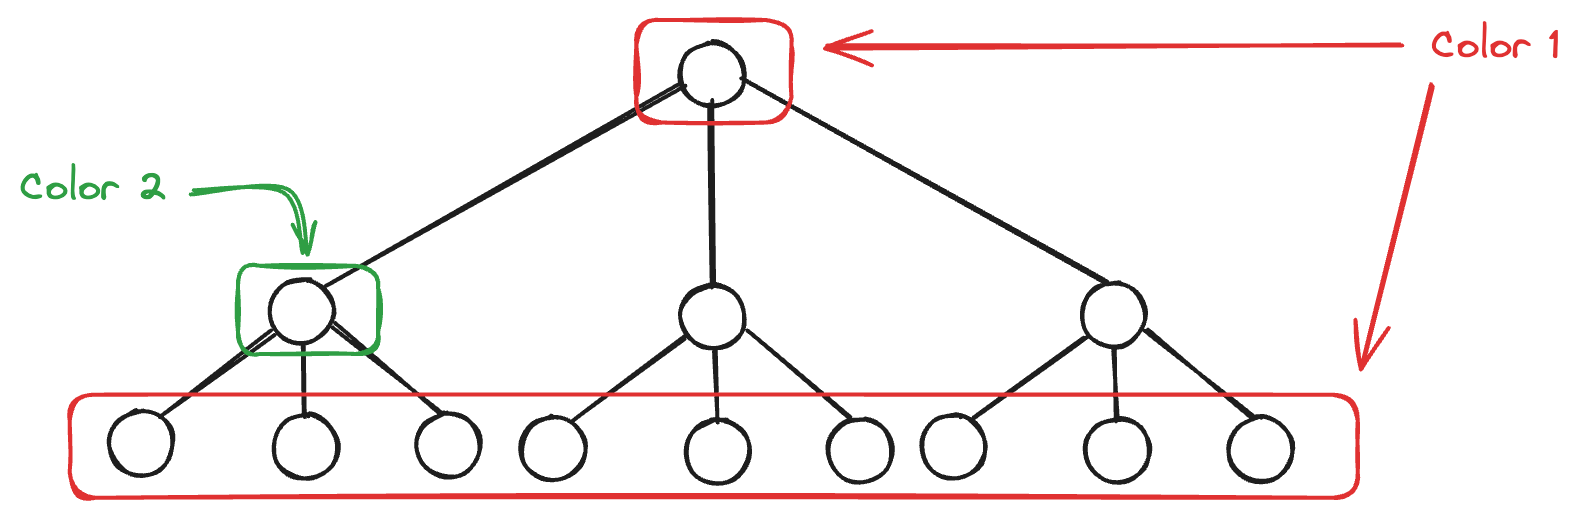
\includegraphics[width=0.7\linewidth]{layer 3.png}
    \caption{For a three layer deep tree only one node can be colored with Color $2$}
    \label{fig:enter-label}
\end{figure}

For a layer $4$ tree, which is a combination of $3$ layer $3$ trees connected with one extra node. This extra node can not be colored with color $2$. Hence total color $2$ needed is three times the total color $2$ in the $3$ layered tree. Same thing is true for layer $5$ tree also because the extra node (top most node) here will be colored with color $1$ as odd layers are colored with color $1$. We see a deviation from this pattern for layer $6$ tree. It has $3$ layer $5$ trees connected by the top most node. The top most node can not be colored with color $1$ as the immediate next node is colored with color $1$. Hence we can color this with color $2$. Now for layer $7$ tree we see another violation. Layer $7$ tree has 3 layer 6 trees connected by the top most node. Three layer $6$ tree all has the top most node colored with color $2$. This can not stay together. Our algorithm would have not colored 2 out of 3 of these nodes with color $2$. Hence total color $2$ nodes are $2$ less of 3 times the color $2$ in layer $6$ tree. From $8, 9 \dots$ and so on we can see a repeat of this coloring property. Hence we can reach a equation to quantify how many nodes are colored with color $2$ in a complete three-ary tree.

\begin{align*}
    A &= [0, 0, 1, -2]\\
    f_2(x) &= A[x \% 4] + 3 \cdot f_2(x - 1)
\end{align*}

We use $f_2(3) = 1$ as the base-case. 

Here $f_2(x)$ denotes number of color $2$ needed for an $x$ layered complete three-ary tree. If we compute this recursion we get one-tenth of the number of color $1$ used.

\begin{lemma}
    Simple greedy heuristic for complete tree packing coloring, colors at most $\frac{1}{10} ^{\text{th}} + 1$ many nodes with color $2$ as compared to color $1$.
\end{lemma}

\begin{proof}
    Induction hypothesis: suppose $f_2(x - 1) = \frac{3}{4} \cdot \displaystyle\sum_{i = 0} ^{x - 2} 3^i$ is the number of color $2$ used by our algorithm for a $x - 1$ layer deep tree. We need to prove $f_2(x) \leq \frac{3}{4} \cdot \displaystyle\sum_{i = 0} ^{x - 1} 3^i$ and verify this with experimental results.

    Using induction hypothesis and previous results we get,
    \begin{align*}
        f_2(x) &= A[x\%4] + 3 \cdot f_2(x - 1)\\
        &= A[x\%4] + 3 \cdot \frac{1}{10} \cdot \frac{3}{4} \cdot \displaystyle\sum_{i = 0} ^{x - 2} 3^i\\
        &= A[x\%4] + \frac{3}{4} \cdot \frac{1}{10} \cdot \displaystyle\sum_{i = 0} ^{x - 1} 3^i\\
    \end{align*}

    Here $A[i] \in \{-2, 0, 1\}$, hence $f_2(x)$ is upper bounded by $1 + \frac{1}{10} \cdot f_1(x)$ where $f_1(x)$ is the number of color $1$ used.
\end{proof}

Using the above lemma we can write the following

\begin{align*}
    A &= [0, 0, 1, -2]\\
    f_2(x) &= A[x \% 4] + 3 \cdot f_2(x - 1)\\
    &= \frac{1}{10} \cdot \frac{3}{4} \cdot \displaystyle\sum_{i = 0} ^{x - 1} 3^i\\
    &= \frac{3}{40} \cdot \displaystyle\sum_{i = 0} ^{x - 1} 3^i
\end{align*}

Careful analysis and observations of the experimental results of the algorithm also shows the following simple provable facts,

\begin{itemize}
    \item For three-ary complete trees number of nodes colored with color $(2, 3), (4, 5), (6, 7), \dots$ are the same pairwise,
    \item For three-ary complete trees number of nodes colored with color $(4, 5),$ is one-third of the number of nodes colored with $(2, 3)$ and so on,
    \item After a while when some pair of colors $(x, x + 1)$ are used $\leq 3$ times, all the colors from $x + 2$ and so on are used only once.
\end{itemize}

\subsection{Total color upper bound}

As we have these numbers indicating the count of nodes colored by some color $x$ we can estimate the upper bound on the number of different colors used by our algorithm.

\begin{theorem}
    Simple greedy heuristic is a $\frac{n}{40}$ approximation algorithm for complete three-ary trees.
\end{theorem}

\begin{proof}
    Say we are coloring an $x$ layer deep complete three ary tree with total number of node $= n, n = \displaystyle\sum_{i = 0} ^{x - 1} 3^i$
    \begin{itemize}
        \item Number of nodes colored with color $1 = \frac{3n}{4}$
        \item Number of nodes colored with color $2, 3 = \frac{3n}{40}$
        \item Number of nodes colored with color $4, 5 = \frac{n}{40}$
        \item Number of nodes colored with color $6, 7 = \frac{n}{120}$
        \item Number of nodes colored with color $8, 9 = \frac{n}{360}$
        \item \dots
    \end{itemize}

    We say $j = 1$ at color $2, 3$, from there on $j$ stops at $j = j$ when $\frac{n}{n} = 1$. From there on rest of all the nodes are colored with an non-reusable color.

    Total number of different colors used $= 1 + 2\cdot j + \textsf{ number of non-reusable colors}$. We now need to calculate the number of non-reusable colors and the value of $j$. Value of $j$ when the denominator becomes $n$ is when re-usable colors are finished.

    \begin{align}
        \textsf{Total uniquely used color} &= n - \left[ \frac{3n}{4} + 2 \cdot \left( \frac{3n}{40} + \frac{n}{40} + \frac{n}{40 * 3} + \frac{n}{40 * 3^2} \dots + 1 \right)\right]
    \end{align}

    First we calculate $\left( \frac{3n}{40} + \frac{n}{40} + \frac{n}{40 * 3} + \frac{n}{40 * 3^2} \dots + 1 \right)$.

    \begin{align*}
        s_n &= \left( \frac{3n}{40} + \frac{n}{40} + \frac{n}{40 * 3} + \frac{n}{40 * 3^2} \dots + 1 \right)\\
        &= \frac{3n}{40} \left[ \frac{1 - \left(\frac{1}{3}\right)^{2 + \log_3\left(\frac{n}{40}\right)}}{1 - \frac{1}{3}} \right]\\
        &= \frac{9n}{80} - \frac{1}{2}
    \end{align*}

    we put this into the equation 3.1, then we get
    \begin{align*}
        &= n - \left[\frac{3n}{4} + 2 \cdot \left(\frac{9n}{80} - \frac{1}{2}\right)\right]\\
        &= \frac{n}{40} + 1
    \end{align*}

    We put this calculation into the original equation to get the total number of colors used as
    \begin{align}
        \textsf{Total colors used} &= 1 + 2 \cdot \left[\log_3\left(\frac{n}{40} + 2\right)\right] + \frac{n}{40} + 1\\
        &\geq \frac{n}{40}
    \end{align}

    For very large $n$ expression 3.2 evaluates to almost $\frac{n}{40}$. This proves our lemma saying, our simple greedy algorithm outputs a valid packing coloring assignment with at-least $\frac{n}{40}$ many colors.
\end{proof}

\section{Experimental Results and future works}

\subsection{Number of colors used}
In this chapter we show the experimental results we obtained by running the algorithm on a complete three-ary tree. Following table shows how many colors are used in a $x$-layer complete three-ary tree.

\begin{table}[h]
\centering
\begin{tabular}{|l|l|l|l|l|}
\hline
\# of Nodes & \# of Layers & X-ary tree & Total Colors & Time\\
\hline
13 & 3 & 3 & 4 & 0ms \\\hline
40 & 4 & 3 & 7 & 0ms \\\hline
121 & 5 & 3 & 11 & 2ms \\\hline
364 & 6 & 3 & 19 & 6.11029 ms \\\hline
1093 & 7 & 3 & 40 & 38ms \\\hline
3280 & 8 & 3 & 98 & 63ms \\\hline
9841 & 9 & 3 & 269 & 1s 101ms \\\hline
29524 & 10 & 3 & 781 & 3s 845ms \\\hline
88573 & 11 & 3 & 2309 & 45s 256ms \\\hline
265720 & 12 & 3 & 6890 & 4m 17s 31ms \\ \hline
7174453 & 15 & 3 & 185525 & 9 days 7 hours 29 min 9 sec\\
\hline
\end{tabular}
\caption{Runtime, total color used for a complete three-ary tree.}
\end{table}

All of the result are bounded from above by $\frac{n}{40}$ for the number of colors used by the algorithm. The runtime of the $15$ layer deep tree is skewed because it was run on a older computer with less compute power. All the other experiments were run on \texttt{Apple Macbook Air, M1} processor with \texttt{8 GB} of RAM.

\subsection{Reusable colors}

\begin{table}
    \centering
    \begin{tabular}{|l|l|}
        \hline
        \# of layers & Last reused color\\\hline
        7 & 9 \\\hline
        8 & 11\\\hline
        9 & 13\\\hline
        10 & 15\\\hline
        15 & 25\\
        \hline
    \end{tabular}
    \caption{Number of re-usable colors used by algorithm}
\end{table}

Here we look at the experimental results as to how many colors are there, that being used more than once. Table 4.2 shows that not more than $2\cdot x + 2$ many colors are reusable in a $x$ layer deep complete three-ary tree. This helps in the optimization \# 3 we discussed last chapter.

\subsection{Reusable Colors and number of nodes colored with it}
In this section we'll look at how many nodes are colored with each of the reusable colors. We'll look into for all the $x$-layer complete three-ary trees what is the number of nodes colored by each of the colors.

\subsubsection{For 3 layer deep tree}
Following is the stat for three layer deep complete three-ary tree.

\begin{table}[h]
    \centering
    \begin{tabular}{|l|l|}
        \hline
        \textbf{Color number} & \textbf{Number of nodes} \\ \hline
        1                     & 10                                           \\ \hline
        2                     & 1                                            \\ \hline
        3                     & 1                                            \\ \hline
        4                     & 1                                            \\ \hline
    \end{tabular}
    \caption{Number of nodes colored with each color for 3 layer deep tree.}
    \label{tab:colors}
\end{table}

\subsubsection{For 4 layer deep tree}
Table $4$ shows the stats for four layer deep complete three-ary tree.

\begin{table}[h]
    \centering
    \begin{tabular}{|l|l|}
        \hline
        \textbf{Color number} & \textbf{Number of nodes} \\ \hline
        1                     & 30                                          \\ \hline
        2                     & 3                                           \\ \hline
        3                     & 3                                           \\ \hline
        4  $\to$ 7                  & 1\\ \hline
    \end{tabular}
    \caption{Number of nodes colored with each color for a 4-layer deep tree.}
    \label{tab:colors}
\end{table}

\subsubsection{For 5 layer deep tree}
Table $5$ shows the stats for 5 layer deep complete three-ary tree.

\begin{table}[h]
    \centering
    \begin{tabular}{|l|l|}
        \hline
        \textbf{Color number} & \textbf{Number of nodes} \\ \hline
        1                     & 91                                          \\ \hline
        2                     & 9                                           \\ \hline
        3                     & 9                                           \\ \hline
        4                     & 3                                           \\ \hline
        5                     & 3                                           \\ \hline
        6  $\to$ 11 & 1                                           \\ \hline
    \end{tabular}
    \caption{Number of nodes colored with each color for a 5-layer complete tree.}
    \label{tab:colors}
\end{table}

\subsubsection{For 6 layer deep tree}
Table $6$ shows the stats for 6 layer deep complete three-ary tree.

\begin{table}[h]
    \centering
    \begin{tabular}{|l|l|}
        \hline
        \textbf{Color number} & \textbf{Number of nodes} \\ \hline
        1                     & 273                                          \\ \hline
        2                     & 28                                           \\ \hline
        3                     & 27                                           \\ \hline
        4                     & 9                                           \\ \hline
        5                     & 9                                           \\ \hline
        6                     & 3                                           \\ \hline
        7                     & 3                                           \\ \hline
        8 $\to$ 19& 1                                           \\ \hline
    \end{tabular}
    \caption{Number of nodes colored with each color for a 6-layer complete tree.}
    \label{tab:colors}
\end{table}

From color $8$ till $19$ all are the colors used only once in the tree.

\subsubsection{For 7 layer deep tree}
Table $7$ shows the stats for 7 layer deep complete three-ary tree.

\begin{table}[h]
    \centering
    \begin{tabular}{|l|l|}
        \hline
        \textbf{Color number} & \textbf{Number of nodes} \\ \hline
        1                     & 820                         \\ \hline
        2                     & 82                         \\ \hline
        3                     & 82                         \\ \hline
        4                     & 27                         \\ \hline
        5                     & 27                         \\ \hline
        6                     & 9                          \\ \hline
        7                     & 9                          \\ \hline
        8                     & 3                          \\ \hline
        9                     & 3                          \\ \hline
        10 $\to$ 40  & 1\\ \hline
    \end{tabular}
    \caption{Number of nodes colored with each color for a 7-layer complete tree.}
    \label{tab:colors}
\end{table}


Total of $40$ colors used by the algorithm, from color $10$ till $40$ all are the colors used only once in the tree.


\subsubsection{For 8 layer deep tree}
Table $8$ shows the stats for 8 layer deep complete three-ary tree.

\begin{table}[h]
    \centering
    \begin{tabular}{|l|l|}
        \hline
        \textbf{Color number} & \textbf{Number of nodes} \\ \hline
        1                      & 2460                      \\ \hline
        2                      & 246                       \\ \hline
        3                      & 246                       \\ \hline
        4                      & 82                        \\ \hline
        5                      & 81                        \\ \hline
        6                      & 27                        \\ \hline
        7                      & 27                        \\ \hline
        8                      & 9                         \\ \hline
        9                      & 9                         \\ \hline
        10                     & 3                         \\ \hline
        11                     & 3                         \\ \hline
        12 $\to$ 98  & 1\\ \hline
    \end{tabular}
    \caption{Number of nodes colored with each color for a 8-layer complete tree.}
    \label{tab:colors}
\end{table}


Total of $98$ colors used by the algorithm, from color $12$ till $98$ all are the colors used only once in the tree.

\subsubsection{For 9 layer deep tree}
Table $9$ shows the stats for 9 layer deep complete three-ary tree. Total of $269$ colors used by the algorithm, from color $14$ till $269$ all are the colors used only once in the tree.

\begin{table}[h]
    \centering
    \begin{tabular}{|l|l|}
        \hline
        \textbf{Color number} & \textbf{Number of nodes} \\ \hline
        1                      & 7381                      \\ \hline
        2, 3                      & 738                       \\ \hline
        4, 5                      & 244                       \\ \hline
        6, 7                      & 81                        \\ \hline
        8, 9                      & 27                        \\ \hline
        10, 11                     & 9                         \\ \hline
        12, 13                     & 3                         \\ \hline
        14 $\to$ 269  & 1\\ \hline
    \end{tabular}
    \caption{Number of nodes colored with each color for a 9-layer complete tree.}
    \label{tab:colors}
\end{table}

\subsubsection{For 15 layer deep tree}
Table $10$ shows the stats for 15 layer deep complete three-ary tree.

\begin{table}[h]
    \centering
    \begin{tabular}{|l|l|}
        \hline
        \textbf{Color number} & \textbf{Number of nodes} \\ \hline
        1                      & 5380840                   \\ \hline
        2, 3                      & 538084                    \\ \hline
        4                      & 177391                    \\ \hline
        5                      & 177390                    \\ \hline
        6, 7                   & 59058                     \\ \hline
        8, 9                   & 19684                     \\ \hline
        10, 11                 & 6561                      \\ \hline
        12, 13                 & 2187                      \\ \hline
        14, 15                 & 729                       \\ \hline
        16, 17                 & 243                       \\ \hline
        18, 19                 & 81                        \\ \hline
        20, 21                 & 27                        \\ \hline
        22, 23                 & 9                         \\ \hline
        24, 25                 & 3                         \\ \hline
        26 $\to$ 185525  & 1\\ \hline
    \end{tabular}
    \caption{Number of nodes colored with each color for a 15-layer complete tree.}
    \label{tab:colors}
\end{table}


Total of $185525$ colors used by the algorithm, from color $26$ till $185525$ all are the colors used only once in the tree.

\subsection{Results on Binary Trees}
As an exercise we've ran our algorithm for Binary Trees. It is known that at most $7$ colors are needed for binary trees to be colored. Here is the data showing how many colors are needed by our algorithm. It is to be noted that this algorithm also outputs a coloring assignment at the end of the runtime. The theoretical upper bound of $7$ does not show us a valid coloring assignment. This is shown in Table 11.

\begin{table}[h]
    \centering
    \begin{tabular}{|c|c|c|c|}
        \hline
        \textbf{Nodes} & \textbf{Layers} & \textbf{Colors used} & \textbf{Total time} \\ \hline
        31 & 5 & 5 & 0ms \\ \hline
        63 & 6 & 9 & 1ms \\ \hline
        127 & 7 & 9 & 1ms \\ \hline
        255 & 8 & 15 & 5ms \\ \hline
        1023 & 10 & 25 & 25ms \\ \hline
        4095 & 12 & 53 & 113ms \\ \hline
        8191 & 13 & 53 & 159ms \\ \hline
        32767 & 15 & 155 & 1s 585ms \\ \hline
        65535 & 16 & 549 & 14s 758ms \\ \hline
        131071 & 17 & 549 & 26s 518ms \\ \hline
        262143 & 18 & 2117 & 3m 54s 261ms \\ \hline
        4194303 & 22 & 2118 & 6m 22s 851ms \\ \hline
    \end{tabular}
    \caption{Binary Tree Coloring assignments}
    \label{tab:data_2}
\end{table}

One very interesting observation we can see that jumping from 18 to 22 layer binary tree it increases extra colors by only $1$. There maybe a plateau for our algorithm for much higher nodes on the number of colors used. This remains to be examined later.


\subsection{Randomized Tree Pruning and performance}
We only analyzed our algorithm performance on complete three-ary trees. Our next goal is to measure the performance for any trees. As a set of objectives we've thought of developing some randomized graph generation scheme according to fixed distributions. This may involve development of very non-trivial and novel approaches in data generation that are yet to be discovered. We here will see a very simple version of that. We'll use this as the foundation for developing very non-trivial randomized graph generation schemes later.

We define the following tree pruning service

\begin{algorithm}[H]\label{alg:2}
    \SetAlgoLined
    \KwIn{Tree $T$, Starting Root $u$, Probability reduction factor $p$}

    Compute the level order traversal of the tree $T$\;
    \texttt{p\_current} $\gets \frac{1}{2}$\;
    \ForEach{level from the last level, going one level up each iteration}{
        \ForEach{Node in this level}{
            Remove this nodes all children with probability \texttt{p\_current}\;
        }
        \texttt{p\_current} $\gets \frac{\texttt{p\_current}}{2}$\;
    }
    
    \KwOut{We are modifying the tree in-place, hence no output required.}
    \caption{\texttt{ModifyTree(Tree $T$, Root $u$)}}
\end{algorithm}

Using this strategy we have the following stats in table $12$ while running our algorithm on those pruned trees. These trees are always $4$ degree bounded, each node either has none or all the children, and very unlikely it is skewed and sparse.

\begin{table}[h]
    \centering
    \begin{tabular}{|c|c|c|c|c|c|}
        \hline
        \textbf{Level} & \textbf{Nodes} & \textbf{Nodes After Pruning} & \textbf{Colors} & \textbf{N/C Ratio} & \textbf{Comments} \\ \hline
        10 & 29524 & 18082 & 80 & 226.025 &  \\ \hline
        10 & 29524 & 17953 & 77 & 233.1558442 & \\ \hline
        10 & 29524 & 18256 & 79 & 231.0886076 & \\ \hline
        10 & 29524 & 18172 & 66 & 275.3333333 & \\ \hline
        10 & 29524 & 18214 & 104 & 175.1346154 & \\ \hline
        10 & 29524 & 18199 & 52 & 349.9807692 & \\ \hline
        10 & 29524 & 29524 & 781 & 37.8028169 & Complete Tree \\ \hline
        & & & & & \\ \hline
        7 & 1093 & 913 & 16 & 57.0625 &  \\ \hline
        7 & 1093 & 898 & 9 & 99.77777778 & \\ \hline
        7 & 1093 & 913 & 14 & 65.21428571 & \\ \hline
        7 & 1093 & 892 & 9 & 99.11111111 & \\ \hline
        7 & 1093 & 1093 & 40 & 27.325 & Complete Tree \\ \hline
        & & & & & \\ \hline
        4 & 40 & 22 & 6 & 3.666666667 &  \\ \hline
        4 & 40 & 28 & 6 & 4.666666667 & \\ \hline
        4 & 40 & 25 & 6 & 4.166666667 & \\ \hline
        4 & 40 & 31 & 7 & 4.428571429 & \\ \hline
        4 & 40 & 40 & 7 & 5.714285714 & Complete Tree \\ \hline
        & & & & & \\ \hline
        9 & 9841 & 8167 & 55 & 148.4909091 & \\ \hline
        9 & 9841 & 8248 & 27 & 305.4814815 & \\ \hline
        9 & 9841 & 8161 & 48 & 170.0208333 & \\ \hline
        9 & 9841 & 8146 & 49 & 166.244898 & \\ \hline
        9 & 9841 & 8152 & 29 & 281.1034483 & \\ \hline
        9 & 9841 & 9841 & 269 & 36.58364312 & Complete Tree \\ \hline
    \end{tabular}
    \caption{Data for different tree levels}
    \label{tab:data}
\end{table}


\section{Future Works and Plans}
In future a lot more need to be examined and significant theories need to be developed for our algorithm,

\begin{itemize}
    \item We analysed our algorithm performance on a complete three-ary tree and some trees with randomly delete branch. We need to analyse the performance for any $d$-degree bounded tree and graphs. To do this one approach we thought of is to design an algorithm that'll find a suitable root such that most of the nodes are equidistant from this root. Suitable root must decrease the number of colors to be used by our algorithm.
    \item To test the effectiveness of the algorithm we need to come up with a random-graph generation scheme. Through which we can generate graphs at random with certain properties and review our algorithm performance.
    \item We need to come up with a randomized graph generation scheme that'll generate worst case graphs to color for our algorithm. This will generate the worst case graphs, that'll cost very significant amount of colors to color according to our coloring strategy and some fix for those graphs. We also need to check the performance of our algorithm on randomly chosen graph from a fixed distribution.
\end{itemize}

\end{document}
